\documentclass[text01.tex]{subfiles}
\begin{document}
%
% section 1.6
%
\section{チャレンジ(できる人はやってみてね)}

%\liststyleLxxx
\begin{itemize}
      \item
            今日作った\ruby{自己}{じこ}\ruby{紹介}{しょうかい}ページを参考にして、
            自分の学校または自分のしゅみなどを\ruby{紹介}{しょうかい}するページを作ろう。

            \begin{itemize}
                  \item ヒント :
                        まずは、01フォルダの中にある\texttt{template.html}をコピーして\texttt{kadai.html}を作ろう。
                  \item ヒント :
                        コピーしたファイルを書き\ruby{換}{か}えていこう。
            \end{itemize}
      \item
            表を使って、学校の\ruby{時間割}{じかんわり}表を作ってみよう。

            \begin{itemize}
                  \item ヒント :
                        まずは、01フォルダの中にある\texttt{template.html}をコピーして\texttt{kadai2.html}を作ろう。
                  \item ヒント :
                        コピーしたファイルを書き\ruby{換}{か}えていこう。
            \end{itemize}
      \item
            タイピングゲームに何度も\ruby{挑戦}{ちょうせん}してタイピングマスターになろう。
      \item 問題をすべて\ruby{解}{と}いてみよう。
\end{itemize}

\begin{figure}[htbp]
      \begin{minipage}[t]{0.55\columnwidth}
            \centering
            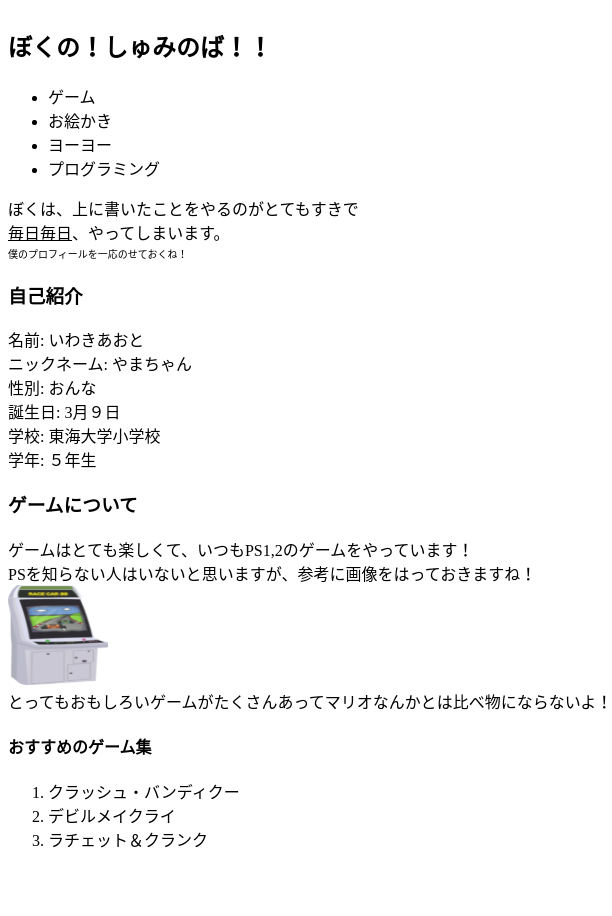
\includegraphics[width=0.9\linewidth]{../../asset/image/textbook-img209.png}
            \caption{自己\ruby{紹介}{しょうかい}ページの例}
      \end{minipage}\hfill
      %
      \begin{minipage}[t]{0.4\columnwidth}
            \centering
            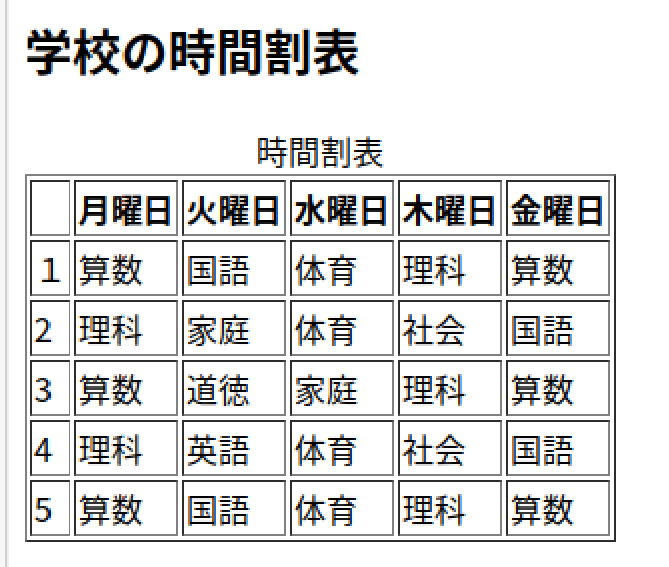
\includegraphics[width=0.9\linewidth]{../../asset/image/textbook-img211.png}
            \caption{\ruby{時間割}{じかんわり}表の例}
      \end{minipage}
\end{figure}
\clearpage

% \begin{figure}[htbp]
%       \centering
%       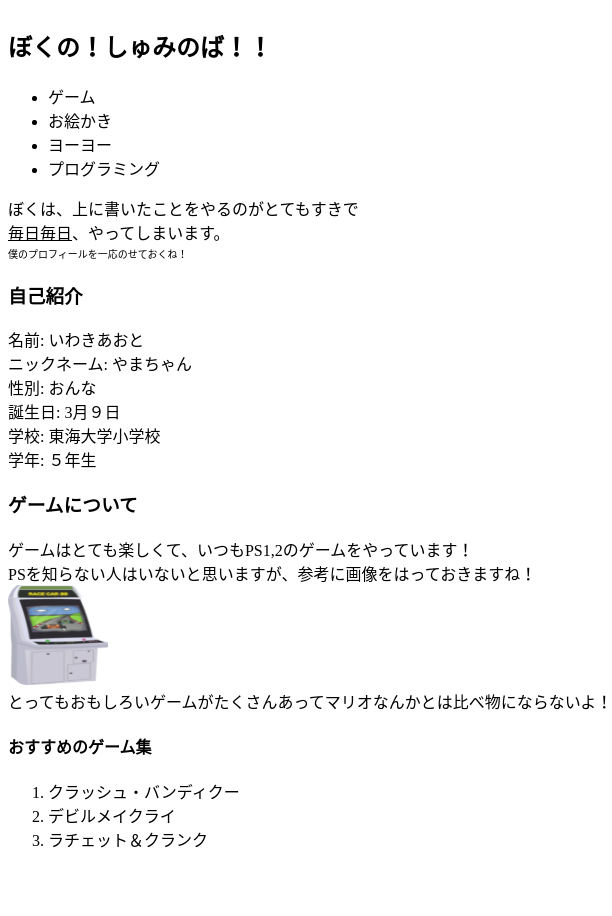
\includegraphics[width=0.9\linewidth]{../../asset/image/textbook-img209.png}
%       \caption{自己\ruby{紹介}{しょうかい}ページの例}
%       \label{fig:1.6.1}
% \end{figure}

% \begin{figure}[htbp]
%       \centering
%       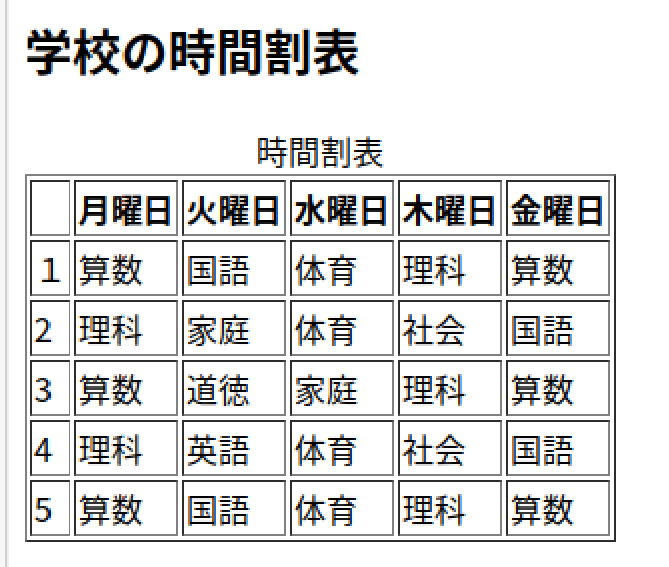
\includegraphics[width=0.9\linewidth]{../../asset/image/textbook-img211.png}
%       \caption{\ruby{時間割}{じかんわり}表の例}
%       \label{fig:1.6.2}
% \end{figure}



\end{document}
